% !TeX root = main.tex

\section{Approche}

	Dans cette partie, nous expliquerons quels sont les différents outils et stratégies mis en place pour permettre la résolution du problème.
	
	La principale difficulté c'est que le jeu de base est trop complexe et ne permet pas de déterminer si l'approche actuelle est mieux adapté. Par conséquent, on utilisera des instances plus petites, qui sont des plateaux de plus petite taille (4x4, 5x5 ...) qui respectent les deux lois d'Eternity II. 
	
	En supposant que la smartforce devient de plus en plus bénéfique suivant la complexité du problème, il est nécessaire de mettre en place une valeur étalon, reposant sur un programme bruteforce qui fournit différentes données permettant d'estimer si l'approche de la smartforce est plus bénéfique.
	
	Chaque n\oe ud de l'arbre des possibilités du jeu doit satisfaire deux données :
	
	\begin{description}
		\item[variable] : une des cases
		\item[valeur] : une des pièces.
	\end{description}
	
	Lors de la progression dans l'arbre, il faut définir quelle valeur sera définie pour quelle variable (choisir telle case sur laquelle sera placée telle pièce). Pour cela, chaque variable (case) possède un domaine de valeur, un tableau contenant contient toutes les valeurs possibles (toutes les pièces qui peuvent être mise dessus) que l'on appellera \textbf{domaine}.
	Et inversement, chaque valeur (pièce) possède un domaine contenant toutes les variable à laquelle elle peux être appliquée.

	\subsection{Bruteforce}
	
	Le programme de bruteforce nous fournit une valeur étalon. Il se contente de parcourir tout l'arbre des possibilités.
	
	Il permet aussi de savoir quelle stratégie de chemin de parcours du plateau est la plus bénéfique. Les différentes stratégies de choix de variables étudiés sont :
	
	\begin{figure}[H]
		\minipage{0.32\textwidth}
		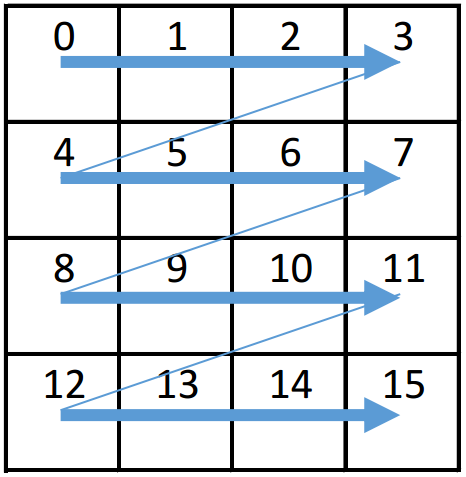
\includegraphics[width=\linewidth]{images/parcours_rowscan.png}
		\caption{\textbf{rowscan} : parcours horizontal du plateau}\label{fig:parcours_rowscan}
		\endminipage\hfill
		\minipage{0.32\textwidth}
		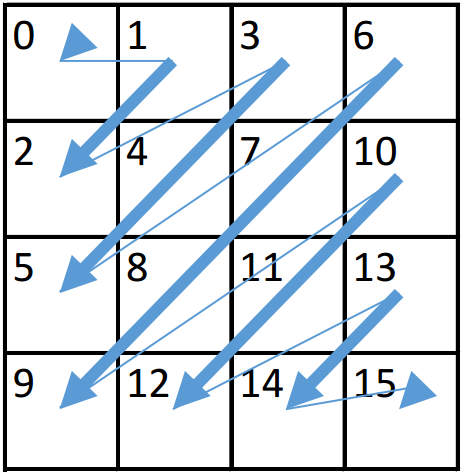
\includegraphics[width=\linewidth]{images/parcours_diagonal.png}
		\caption{\textbf{diagonal} : parcours diagonal du plateau}\label{fig:parcours_diagonal}
		\endminipage\hfill
		\minipage{0.32\textwidth}
		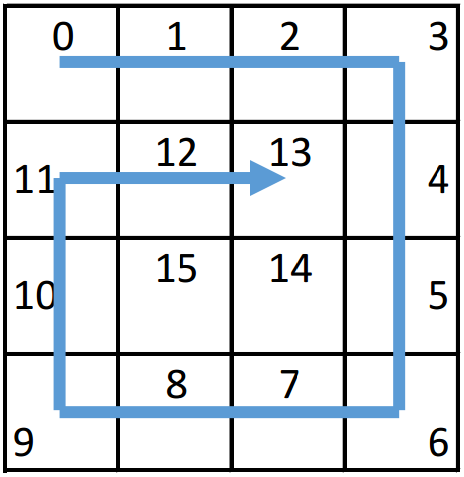
\includegraphics[width=\linewidth]{images/parcours_spiral-in.png}
		\caption{\textbf{spiral-in} : parcours en spirale fermente du plateau}\label{fig:parcours_spiral-in}
		\endminipage\hfill
	\end{figure}
	\begin{figure}[H]
		\minipage{0.32\textwidth}
		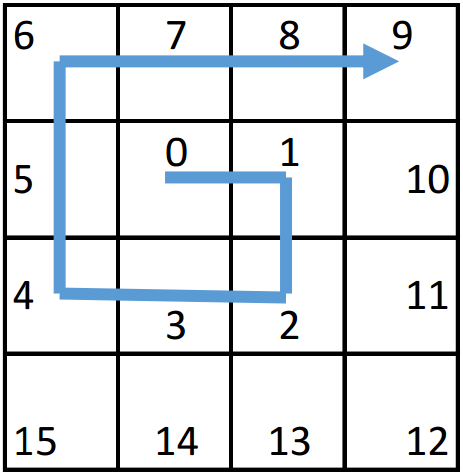
\includegraphics[width=\linewidth]{images/parcours_spiral-out.png}
		\caption{\textbf{diagonal} : parcours en spirale ouvrante du plateau}\label{fig:parcours_spiral-out}
		\endminipage\hfill
		\minipage{0.32\textwidth}
		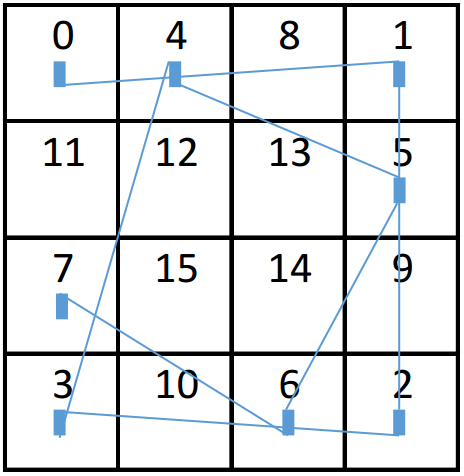
\includegraphics[width=\linewidth]{images/parcours_quad-spiral-in.png}
		\caption{\textbf{quad spiral out} : parcours avec quatre spirales fermentes}\label{fig:quad-spiral-in}
		\endminipage\hfill
		\minipage{0.32\textwidth}
		\ %don't touch this !
		\endminipage\hfill
	\end{figure}
	
	Le choix des pièces (valeurs) est fait dans l'ordre lexicographique.
	
	Les données utilisés pour l'étalonnage sont les suivants :
	
	\begin{description}
		\item[Première solution] : le temps et la quantité de n\oe uds nécessaires pour trouver la première solution (chaque instance peux en avoir plusieurs)
		\item[Nombre total de solutions] : pour estimer les placement des solutions dans l'arbre
		\item[Nombre total de n\oe uds] : pour pouvoir estimer la rapidité de l'algorithme pour trouver la première solution
		\item[Temps total] : pour connaître si l'algorithme utilisé est plus performant que celui d'avant
	\end{description}
	
	--- [résumé]
	
	Afin de pouvoir partir sur de bonnes bases, plusieurs différents méthodes de parcours (quel chemin prendre pour résoudre mon plateau) ont été utilisé, afin de voir quel parcours est le plus performant pour la résolution brute. En sachant que le nombre de noeuds/sec est la même, l'unité de mesure est le nombre de noeuds.

	Les différents types de parcours sont :

	\begin{description}
		\item[rowscan]: on pose les pieces en lignes horizontales sur le plateau
		\item[diagonal]: on pose les pieces en diagonal
		\item[spiral in]: on dispose les pièces en spirale en partant de l'exterieur
		\item[spiral out]: idem que spiral in mais en partant de l'intérieur vers l'extérieur
	\end{description}

	Ces différents types de parcours ont été testés sur plusieurs instances de taille variable.

	\subsection{Smartforce}

	La smartforce repose sur la quantité de données qu'elle possède. Par conséquent, il est important que ces données soient bien organisés, afin de pouvoir les traiter avec aise. Ces données sont organisés pour former des modèles. Chaque modèle peut être interprété comme un point de vue différent par rapport au problème.
	
	On note aussi l'introduction de nouvelles méthodes de parcours :
	
	\begin{itemize}
		\item Choix de variable :
		\begin{itemize}
			\item\textbf{Optimiste} : on choisit la variable qui à le plus grand domaine
			\item\textbf{Pessimiste} : on choisit la variable qui à le plus petit domaine
		\end{itemize}
		\item Choix de valeur :
		\begin{itemize}
			\item \textbf{Lexicographique} : utilisé par défaut par la bruteforce, on choisit la valeur suivante dans l'ordre par défaut.
			\item \textbf{Optimiste} : la valeur dont le domaine est le plus grand
			\item \textbf{Pessimiste} : la valeur dont le domaine est le plus petit
		\end{itemize}
	\end{itemize}
	
	Différents modèles seront donc présentés par ordre de difficulté, car, afin de fournir des types de données variés, il est nécessaire d'abstraire le problème initial.
	
--- [résumé]

	Une fois la valeur étalon fixée, il est maintenant facile de mettre en place un autre approche du problème qui à pour principe de cumuler une grande quantité de donnée pour faire face au nombre exponentiel de possibilités.

	Les différents types de données (nommés modèles) sont comme différents points de vues du problème. Ils sont plus ou moins utiles, mais la force réside dans leur union. Mais surtout, ils permettent de mettre en place le concept d'ouvertures et finales.

	\subsubsection{CaPi}

	CaPi est le plus simple modèle représentant le problème. Il à pour variable les cases (identifiés par un numéro ou par ses coordonnées sur le plateau) et pour valeur les pièces (identifiés par un numéro et par leurs rotation). C'est aussi lui qui est utilisé comme modèle par défaut pour le choix des valeurs et variables.
	
	En somme, chaque pièce est associé aux cases sur laquelle elle peut être posée et inversement, chaque case contient la liste des pièces qu'elle peux avoir.
	
	\begin{rem}
		Le domaine des cases est un peu plus complexe : une pièce donnée peux être placée sur la case \enquote{jusqu'à 4 fois} (à plusieurs rotation différentes). Par conséquent, lorsque l'on met à jour le domaine de la case (en posant la pièce sur une autre case), on supprime toutes les occurrences de cette pièce du domaine en question.
		
		Par conséquent, chaque pièce possède en vérité quatre domaines distincts (correspondant à chaque rotation de la pièce).
	\end{rem}

--- [résumé]

	L'approche CaPi (abbréviation de Cases/pieces) est l'approche la plus naive, elle permet de définir quelle piece peut être placée sur telle case et inversement, quelle case peux avoir telle piece.

	Cette approche est l'interaction la plus basique de notre problème. C'est aussi celle-ci qui est utilisée en bruteforce.

	\subsubsection{BoCo}
	
	Le modèle BoCo (Bordures/Couleurs) est une approche bien plus fine, elle découle de l'abstraction de CaPi.
	
	Si l'on connait le domaine d'une case. On connaît les pièces qui peuvent être posés dessus. Par conséquent, on définit une \textbf{Bordure} comme une sous-partie d'une case.
	
	\begin{exmp}
		Prenons la case 0, en 0,0 sur le plateau. Elle peux contenir 4 pièces (\no 0,1,2,3 ; ce sont toutes des pièces de coin) à la rotation 0.
		
		\minipage[t]{0.29\textwidth}
		Si l'on décompose la case, celle-ci contient 4 faces :
		
		\begin{figure}[H]
			\includestandalone[width=\linewidth]{graphics/case}

			\caption{Détails d'une case}\label{fig:case}
		\end{figure}
		
		Les bords 1 et 2 étant gris, il n'est pas nécessaire de les représenter. 
		\endminipage\hfill
		\minipage[t]{0.29\textwidth}
	
		On décompose ensuite les 4 pièces :
		\begin{figure}[H]
			\includestandalone[width=\linewidth]{graphics/4_pieces}
			
			\caption{Couleurs des 4 pièces}\label{fig:4_pieces}
		\end{figure}
		\endminipage\hfill
		\minipage[t]{0.29\textwidth}
			On associe ensuite les couleurs et leur occurence à chaque bord :
			\begin{figure}[H]
				\includestandalone[width=\linewidth]{graphics/4_pieces_on_bordure}
				
				\caption{Occurrences et couleurs de bordures}\label{fig:4_pieces_on_bordure}
			\end{figure}
		\endminipage\hfill
	\end{exmp}
	
	Cette simplification du problème nous permet de connaître plus simplement si deux cases adjacentes possèdent des matching non possibles.  Il suffit ensuite d'éliminer les pièces possèdent la couleur manquante.
		
	\begin{exmp} Dans cet exemple, pour le deuxième cas [\autoref{fig:bordure_no_match}], toutes les pièces (orientés) ayant du rouge sur la face 2 ne peuvent être posés sur la case. Cela vaut aussi pour la case adjacente où la couleur verte ne peux être posée.
			
		\minipage[t]{0.45\textwidth}
			Les deux cases ont des matching possibles :
			
			\begin{figure}[H]
				\includestandalone[width=\linewidth]{graphics/bordure_match}
				\caption{Cases adjacentes avec matching possible}\label{fig:bordure_match}
			\end{figure}
		
		\endminipage\hfill
		\minipage[t]{0.45\textwidth}
			Les deux cases ont des matching non possibles
			
			\begin{figure}[H]
				\includestandalone[width=\linewidth]{graphics/bordure_no_match}
				
				\caption{Cases ayant des matching non possibles}\label{fig:bordure_no_match}
			\end{figure}
			\endminipage\hfill
	\end{exmp}
	
	Les bordures sont identifiés par un numéro. Chaque \textbf{bordure} possède un domaine contenant les \textbf{couleurs} uniques qu'elle peux avoir et leur cardinalité [\autoref{fig:4_pieces_on_bordure}].
	
	Les couleurs sont aussi identifiés par un numéro. Chaque \textbf{couleur} contient l'ensemble des bordures où elle peux être placée, et combien de fois elle peux l'être (cardinalité).
	
	L'utilité de ce modèle réside dans la propagation des données. Le but étant de propager une information à travers les cases, en ne mettant à jour que les données concernées.
	
	Dans une disposition CaPi, pour appliquer la propagation des données, on est obligé de faire le produit des domaines des cases adjacentes pour chaque matching (comparer les pièces possibles de chaque case entre eux). Ce qui s'avère très couteux et beaucoup de ces vérifications sont inutiles.
	
	Par contre, grâce à \textbf{BoCo}, il suffit de vérifier que la cardinalité des couleurs reste positive pour les deux bordures adjacentes. Seulement lorsque le nombre d'occurrences d'une couleur tombe à zéro, l'autre est invalidée (disons, la couleur rouge). Il suffit ensuite de récupérer les autres couleurs de la pièce qui disparait (car elle avait la couleur rouge), et de décrémenter les autres bordures de la case concernée. Si leur occurrence tombe à zéro, on met à jour leur bordure adjacente, sinon, la propagation s'arrête.
	
	--- [résumé]

	L'approche BoCo (Bordure/Couleur) est bien plus fine : si l'on connait quelle piece est sur telle case, on sait quelle couleur peux se placer sur telle bordure [de la case]. Elle permet d'implémenter un système de mis à jour bien plus performant car ne nombre de couleurs est bien plus petit que le nombre de pièces.

	\begin{exmp}
		Si une couleur disparait, alors tt les pièces ayant cette couleur ne peuvent plus être placés à cette case, par conséquent, les autres bords de la case ont (probablement) des couleurs qui disparaissent aussi (propagation de la disparition).
	\end{exmp}

	\subsubsection{Corolles}


	Une corolle est une surface du plateau qui est pré-calculée afin de pouvoir être réutilisée par la suite.
		
	La corolle possède une pièce centrale, de laquelle sont calculées les pièces avoisinantes. Par conséquent, la taille de la corolle est définie par la distance de la pièce la plus au bord par rapport à la pièce centrale, cette distance sera appelée hamming ($H$).
	
	\begin{rem}
		Une corolle de hamming 0 est la pièce elle-même.
	\end{rem}
		
	\begin{figure}[H]
		\begin{minipage}[t]{0.33\textwidth}
			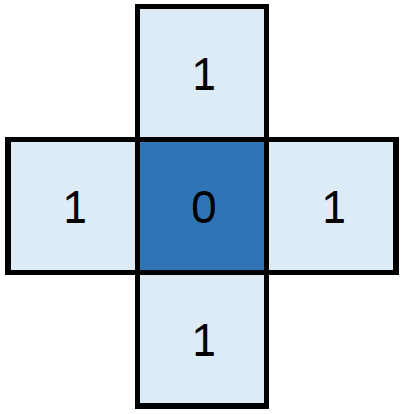
\includegraphics[width=\linewidth]{images/corolle_hamming_1.png}
			\caption{Corolle de hamming 1}\label{fig:corolle_hamming_1}
		\end{minipage}\hfill
		\begin{minipage}[t]{0.33\textwidth}
			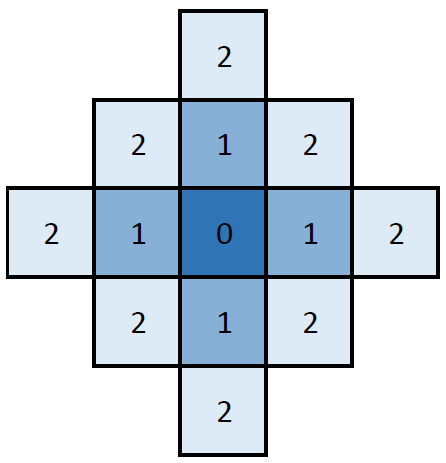
\includegraphics[width=\linewidth]{images/corolle_hamming_2.png}
			\caption{Corolle de hamming 2}\label{fig:corolle_hamming_2}
		\end{minipage}\hfill
		\begin{minipage}[t]{0.33\textwidth}
			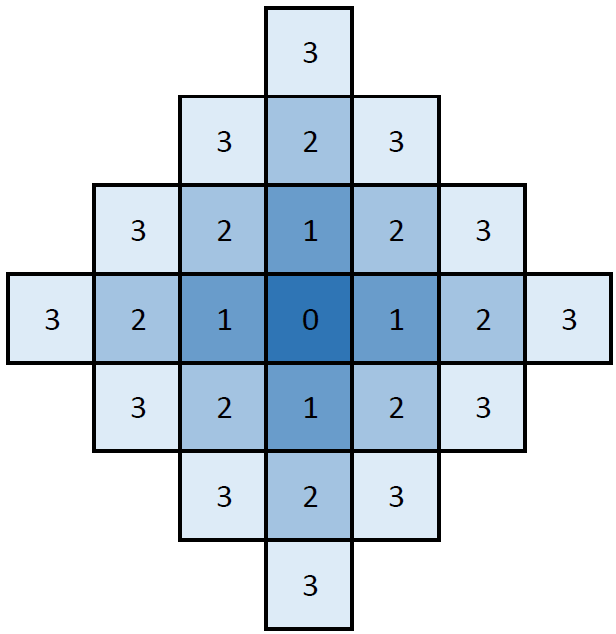
\includegraphics[width=\linewidth]{images/corolle_hamming_3.png}
			\caption{Corolle de hamming 3}\label{fig:corolle_hamming_3}
		\end{minipage}\hfill
	\end{figure}

	Son nom, corolle, vient de sa forme. Suivant son placement, cette forme change. Les différentes formes dépendent de la taille de la corolle (\enquote{rayon} de la corolle) et de la position sur le plateau.
		
	\begin{figure}[H]
		\begin{minipage}[t]{0.33\textwidth}
			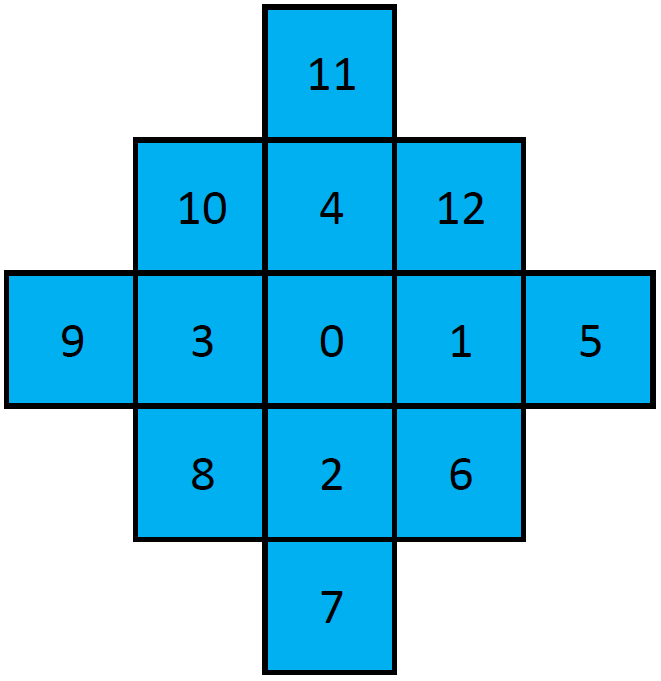
\includegraphics[width=\linewidth]{images/corolle_simple.png}
			\caption{Forme basique d'une corolle}\label{fig:corolle}
		\end{minipage}\hfill
		\begin{minipage}[t]{0.66\textwidth}
			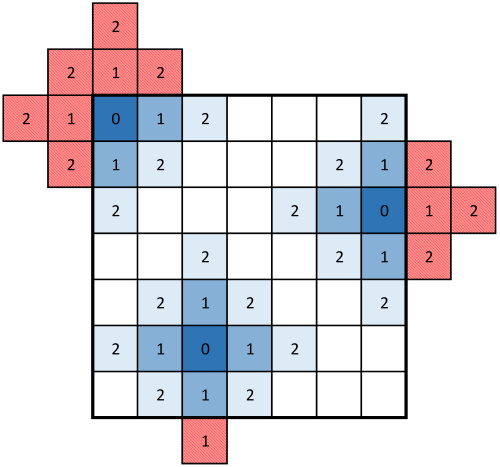
\includegraphics[width=\linewidth]{images/corolle_formes.png}
			\caption{Différentes formes de la corolle de hamming 2 sur une instance de taille 7}\label{fig:corolle_forme}
		\end{minipage}\hfill
	\end{figure}
	
	\begin{exmp}
		Supposons qu'une corolle est seulement définie par sa forme. Prenons comme coordonnées $(0,1)$ et $(1,0)$ avec un hamming de 1. La forme des corolles sur ces coordonnées est identique. Elle à une forme de tétris.
		
		Par conséquent, les corolle en coordonnées $(0,1)$ peuvent aller en $(1,0)$ et inversement.
		
		\begin{figure}[H]
			\begin{minipage}{0.33\textwidth}
				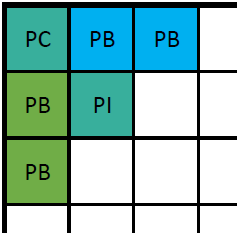
\includegraphics[width=\linewidth]{images/corolle_tetris_bord.png}
				\caption{Corolle en $(0,1)$ (blue)et en $(1,0)$ (vert)}\label{fig:corolle_tetris_bord}
			\end{minipage}\hfill
			\begin{minipage}{0.33\textwidth}
				\begin{center}
					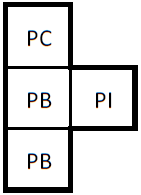
\includegraphics{images/corolle_tetris_1.png}
					\caption{Corolle tetris en $(1,0)$}\label{fig:corolle_tetris_1}
					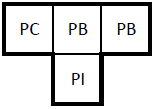
\includegraphics{images/corolle_tetris_2.png}
					\caption{Corolle tetris en $(0,1)$}\label{fig:corolle_tetris_2}
				\end{center}
			\end{minipage}\hfill
			\begin{minipage}{0.33\textwidth}
				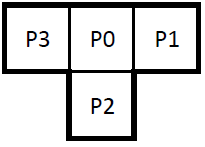
\includegraphics{images/corolle_tetris.png}
				\caption{Noms des pièces dans la corolle tetris}\label{fig:corolle_tetris}
			\end{minipage}\hfill
		\end{figure}
		Or, pour les types de pièces, il y a un problème. en $(1,0)$ P3 est une pièce de coin, alors qu'en $(0,1)$ c'est une pièce de bord (même problème pour P1).
		
		Donc, non seulement, une corolle est définie par sa forme, mais aussi par sa position.
	\end{exmp}
	
	Par conséquent, une corolle est définie par le type de pièces (coin, bord, intérieur) qui la composent et de sa forme. Par conséquent, il n'est pas nécessaire de pré-calculer les corolles sur toutes les cases du plateau. On peux départager le plateaux en zone. Toutes les corolles d'une même zone sont identiques.
	
	\begin{rem}
		Plus le hamming de la corolle augmente, plus il y a des zones différentes à cause de l'augmentation des types de pièces qui la compose.
	\end{rem}
	
	\begin{figure}[H]
		\begin{minipage}{0.49\textwidth}
			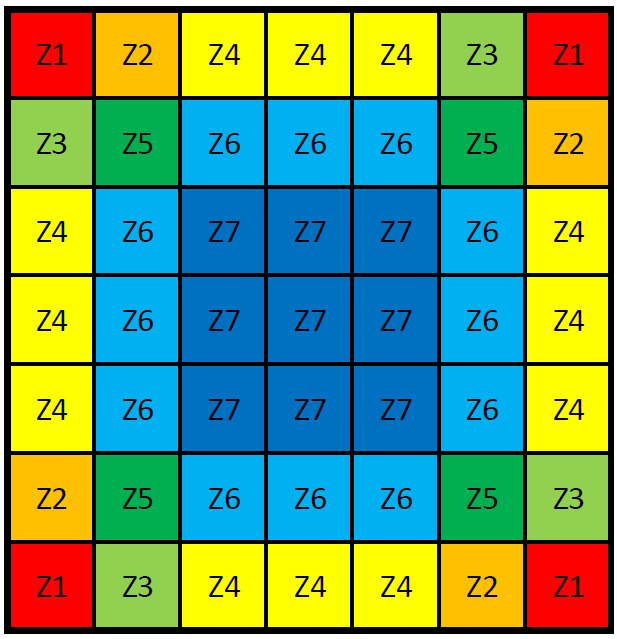
\includegraphics[width=\linewidth]{images/corolle_zones_h_1.png}
			\caption{Quantité de zones differentes sur un plateau de taille 7, pour une corolle de hamming 1}\label{fig:corolle_zones_h_1}
		\end{minipage}\hfill
		\begin{minipage}{0.49\textwidth}
			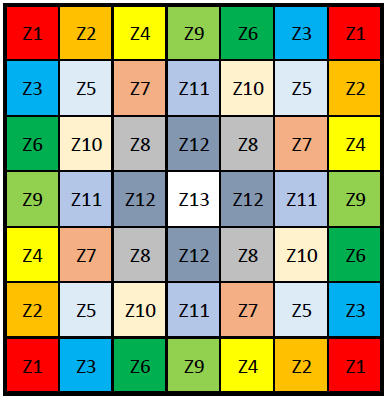
\includegraphics[width=\linewidth]{images/corolle_zones_h_2.png}
			\caption{Quantité de zones différentes sur un plateau de taille 7, pour une corolle de hamming 2}\label{fig:corolle_zones_h_2}
		\end{minipage}\hfill
	\end{figure}
	
	
	\begin{defn}
	Pour tout corolle ayant pour pièce centrale $P$ de taille $H$ d'une zone $Z_1$ donnée, elle découle de l'expansion d'une corolle de
	taille inférieure $H-1$ ayant pour zone $Z_0$ englobant la zone $Z_1$ avec $P$ identique.
	\end{defn}
	
	\begin{defn}
		Une corolle de hamming 2 (H2) contient une corolle de H1 de la zone qui est englobée par la zone de H1
	\end{defn}
	\begin{exmp}
		Dans la ~\autoref{fig:corolle_zones_h_2}, les zones 8,12,13 sont englobées par la zone 7 de H1 [\autoref{fig:corolle_zones_h_1}].
	\end{exmp}

	La frontière définit les couleurs au bord de la corolle, ils sont nécessaires pour connaitre les pièces qui peuvent être placés à côté.
	
	\begin{exmp}
		Les faces d'une couleurs sont la frontière d'une corolle de hamming 0.
	\end{exmp}
	
	Pour résumer. Une corolle est une surface du plateau d'une certaine forme qui est pré-calculée. Une corolle pouvant être à plusieurs endroit, elle set dépendante d'une zone. Elle est composée d'une pièce principale qui la définit ainsi que d'une frontière. Une corolle est composée d'une corolle de hamming inférieur, se trouvant dans une zone englobant la celle de la corolle actuelle.
	
	Afin que la corolle soit correcte, il est nécessaire de connaître les informations suivantes :
	\begin{itemize}
		\item taille du plateau
		\item zone de la corolle
		\item son hamming
		\item les pièces qui la composent
	\end{itemize}
	
	Par la suite, on nommera \textbf{corolle}, l'ensemble des corolles qui ont pour même valeur:
	
	\begin{itemize}
		\item la taille du plateau
		\item zone de la corolle
		\item hamming
		\item pièce principale (et sa rotation).
	\end{itemize}
	
	Cela permet d'utiliser le terme corolle pour nommer un ensemble de toutes les cas possibles lorsque l'on \enquote{pose} une corolle sur le plateau.
	
	--- [résumé]

	Grace aux modèles CaPi et BoCo, il est possible de pré-calculer des zones du plateau nommés corolles, ceux-ci contiennent tous les cas possibles dans cette zone donnée.

	Le nombre de cas possible étant très important, il est nécessaire de le classer. Les corolles peuvent êtres identifiés grâce à plusieurs critères.

	\begin{itemize}
		\item taille du plateau
		\item l'orientation de la corolle
		\item La pièce (et sa rotation) à l'origine de la corolle
		\item La case à l'origine de la corolle
		\item La taille de la corolle
	\end{itemize}

	\subsubsection{BoCoDiag}
	
	%todo